\subsubsection{NDSI Visualization}
The NDSI index measures the relationship between the biophony and the anthrophony of a recording. This is elaborated on in the Overview of Indices section of this report. Because the NDSI is used for comparing two different variables, the representation for this index is different from that of ACI or ADI. Here, two bar charts have been chosen: one for comparing the values per channel, and another for comparing the values side by side. In addition, two line graphs are available for observing the NDSI values along with the biophony and anthrophony for data sets comprised of multiple files, and for analyzing these values at their respective date and time.\par

\begin{center}
  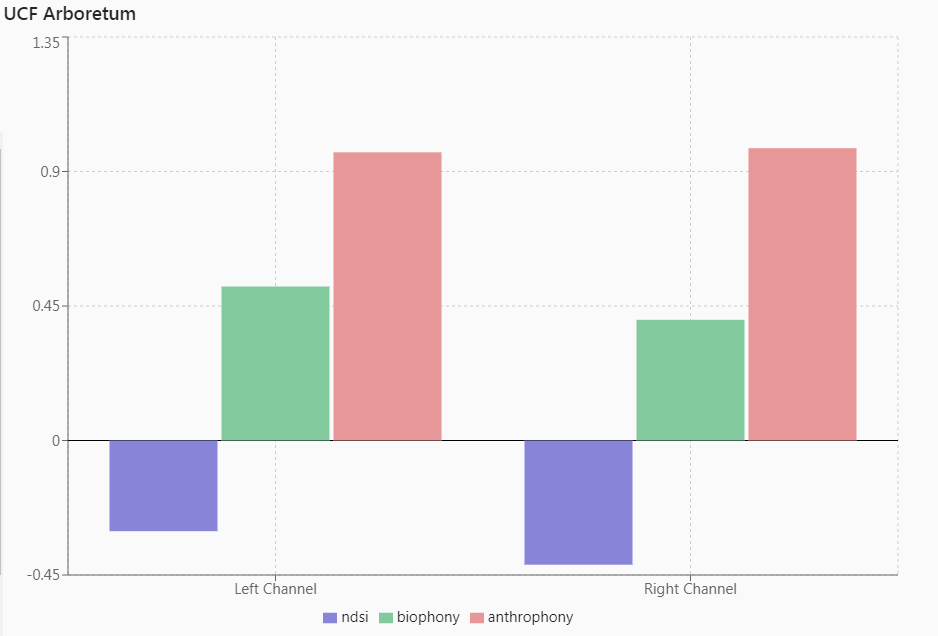
\includegraphics[width=\textwidth]{NDSIgraph1} \\[12pt]
\end{center}
The first visualization available is a bar graph comparing the two channels. Each channel has an overall NDSI value, along with biophony and anthrophony values. Because the NDSI is a difference of the anthrophony and biophony, it is useful to view them side by side in this way. The user is also able to hover over any bar and see the respective data values as they please.\par

\begin{center}
  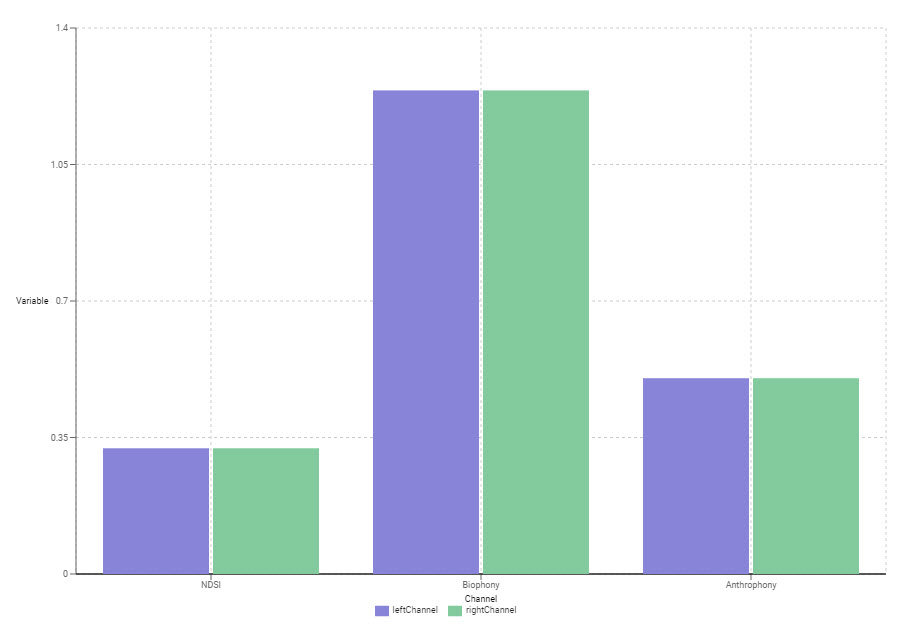
\includegraphics[width=\textwidth]{NDSIgraph2} \\[12pt]
\end{center}
The other visualization available is another bar graph, this one showing the NDSI values, anthrophony values, and biophony values side by side, sorted by channel this time. This representation is useful because often times one channel of the microphone gets different data than the other, and so being able to identify which channel has these differences is helpful for research.\par

\begin{center}
  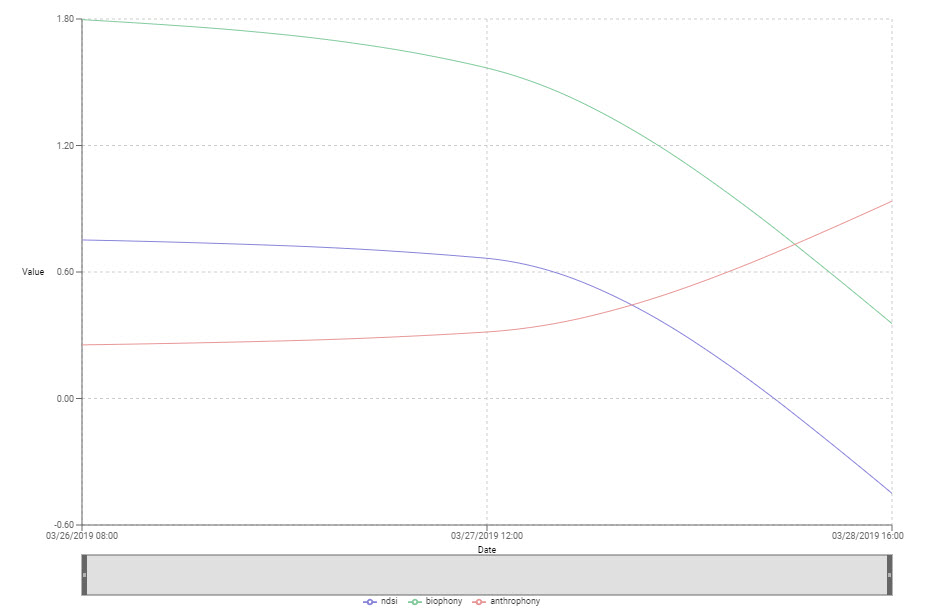
\includegraphics[width=\textwidth]{NDSIgraph3} \\[12pt]
\end{center}
The line graphs available for NDSI value show the NDSI, anthrophony, and biophony by date and time. Researchers often record at different times of day in order to see how index values compare through out the day.\par

\begin{center}
  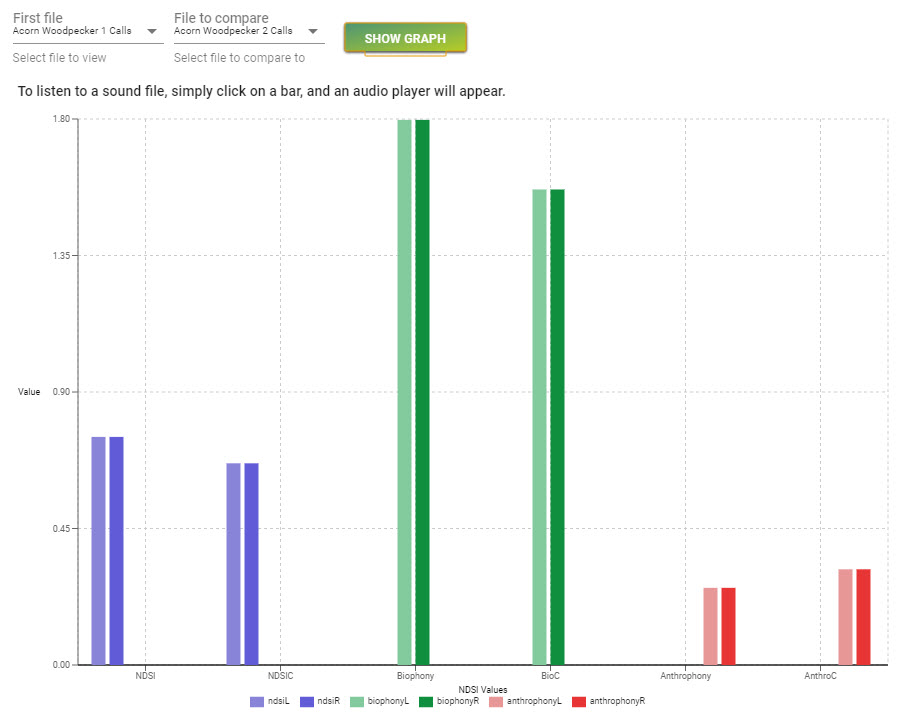
\includegraphics[width=\textwidth]{NDSIgraph4} \\[12pt]
\end{center}
This graph is used to view any individual file in the selected Site and/or Series. This allows for a closer look at what is going on in the data, and also allows you to compare them to other files in the data set, as seen in the image above. With this graph, the user can select a bar chart and an audio player will appear for the user to listen to that file in the client.
